\documentclass[12pt]{article}

\usepackage{array}
\usepackage{amsmath}
\usepackage{amssymb}
\usepackage{mathtools}
\usepackage{textcomp}
\usepackage{gensymb}
\usepackage{graphicx}
\usepackage{float}
\usepackage{caption}
\usepackage{amsfonts}
\usepackage[margin=1in]{geometry}
% \newcommand\df[1]{\index{#1@\myupper #1}{{\bf{#1}}}}
% \newcommand\myupper[1]{\uppercase{#1}}

% \newcommand\myscalar[1]{#1}
\newcommand\myvector[1]{\mathbf{#1}}
\newcommand\mymatrix[1]{\mathbf{#1}}

% \newcommand\mytensor[1]{{\textit{\textsf{\uppercase{#1}}}}}

% \newcommand\myrvscalar[1]{\textrm{#1}}
% \newcommand\myrvvector[1]{\textbf{#1}}
% \newcommand\myrvmatrix[1]{{\textbf{\uppercase{#1}}}}
% \newcommand\myrvtensor[1]{{{\textsf{\uppercase{#1}}}}}

% \newcommand\gup[1]{\textrm{\greektext p}}




\newcommand{\df}[2][]{%
  \ifthenelse{\isempty{#1}}%
    {\index{#2@\myupper #2}{{\bf{#2}}}}% if #1 is empty
    {\index{#2@\myupper #1}{{\bf{#2}}}}% if #1 is not empty
}
\newcommand\myupper[1]{\uppercase{#1}}



\newcommand\twobytwo[4]{\left[\begin{array}{cc}
#1 & #2 \\
#3 & #4 
\end{array}\right]}

\newcommand{\intR}{\int_{-\infty}^{\infty}}
\newcommand{\bounds}[2]{\biggr\rvert_{#1}^{#2}}
\newcommand{\eval}[1]{\biggr\rvert_{#1}}
\newcommand{\opp}[1]{\mathrm{\bf{#1}}}

\newcommand{\Lim}[1]{\raisebox{0.5ex}{\scalebox{0.8}{$\displaystyle \lim_{#1}\;$}}}

\let\origref=\ref

\renewcommand{\ref}[1]{(\origref{#1})}
\newcounter{results}
\newcounter{questions}

\def\neg{{\sim}}
\def\Z{\mathbb{Z}}
\def\N{\mathbb{N}}
\def\R{\mathbb{R}}
\def\Q{\mathbb{Q}}
\def\E{\mathbb{E}}
\def\qed{\(\blacksquare\)}
\newcommand{\result}[1]{\stepcounter{results}{\bfseries Result \arabic{results}}: #1}
\newcommand{\question}[1]{\stepcounter{questions}{\bf \arabic{questions}}: #1}


% %%%%%%%%%%%%%%%%%%%%%%%%%%%%%
% \newenvironment{theorem}[1][Theorem]{\begin{trivlist}
%     \item[\hskip \labelsep {\bfseries #1}] \itshape}{\end{trivlist}}
% \newenvironment{corollary}[1][Corollary]{\begin{trivlist}
%     \item[\hskip \labelsep {\bfseries #1}] \itshape}{\end{trivlist}}
% \newenvironment{example}[1][Example]{\begin{trivlist}
%     \item[\hskip \labelsep {\bfseries #1}] \itshape}{\end{trivlist}}
% %%%%%%%%%%%%%%%%%%%%%%%%%%%%%

% \renewcommand{\qedsymbol}{$\blacksquare$}


\newtheorem{theorem}{Theorem}[section]
\newtheorem{lemma}[theorem]{Lemma}
\newtheorem{proposition}[theorem]{Proposition}
\newtheorem{corollary}[theorem]{Corollary}

\renewenvironment{proof}[1][Proof]{\begin{trivlist}
\item[\hskip \labelsep {\bfseries #1}]}{\qed\end{trivlist}}

\newenvironment{definition}[1][Definition]{\begin{trivlist}
\item[\hskip \labelsep {\bfseries #1}]}{\end{trivlist}}


\newenvironment{remark}[1][Remark]{\begin{trivlist}
\item[\hskip \labelsep {\bfseries #1}]}{\end{trivlist}}


\newcounter{example}
\newenvironment{example}[1][Example]{\refstepcounter{example}\begin{trivlist}
\item[\hskip \labelsep {\bfseries #1~\thesection.\theexample}]}{\end{trivlist}}

\newenvironment{solution}[1][Solution]{\begin{trivlist}
\item[\hskip \labelsep {\bfseries #1}]}{\end{trivlist}}


\renewcommand{\qed}{\nobreak \ifvmode \relax \else
      \ifdim\lastskip<1.5em \hskip-\lastskip
      \hskip1.5em plus0em minus0.5em \fi \nobreak
      \vrule height0.75em width0.5em depth0.25em\fi}
     
     
% \renewcommand{\endsolution}{\nobreak \ifvmode \relax \else
%       \ifdim\lastskip<1.5em \hskip-\lastskip
%       \hskip1.5em plus0em minus0.5em \fi \nobreak
%       \vrule height0.75em width0.5em depth0.25em\fi}    




\title{Green's Functions}
\author{Ryan Coyne}
\date{\today}
\numberwithin{equation}{section}
\numberwithin{figure}{section}
\makeindex

\begin{document}

\maketitle

\tableofcontents

\newpage

\section{Introduction}
The first part of this text is primarily concerned with solutions to differential equations of the form
\begin{equation}
    Lu=\phi
\end{equation}
over an interval \(a \leq x \leq b\) and subject to certain boundary conditions, where \(L\) is an \(n\)th order linear ordinary differential operator, and \(u\) and \(\phi\) are functions of the independent variable. For \(L\) to be linear, it must satisfy the condition
\begin{equation}
	L(\alpha v + \beta w) = \alpha Lv + \beta Lw
\end{equation}
for arbitrary functions \(v\) and \(w\), with \(\alpha\) and \(\beta\) being constant. We claim without proof that for this condition to be met, \(L\) must be of the form
\begin{equation} 
	L = a_0(x) \frac{d^n}{dx^n} + a_1(x) \frac{d^{n-1}}{dx^{n-1}} + \cdots + a_n(x).
\end{equation}
Since \(L\) is of order \(n\), there will be \(n\) boundary conditions of the general form 
\begin{equation}
	B_j (u) = c_j;\quad j=1,2,\dots,n
\end{equation}
where the \(B_j\)'s are prescribed functionals and \(c_j\)'s are prescribed constants. We will only consider \(B_j\)'s that are linear combinations of \(u\) and its derivatives through order \(n-1\) and evaluated at the endpoints, a and b. 

Here, functional refers to a transformation with a set of functions as its domain and a set of numbers as its range. To illustrate what we mean, consider the functional 
\begin{equation}
	\mathcal{F}(u) = \int_{0}^{1} u^2(x)dx.
\end{equation}
The domain of this functional might be the set of functions defined over the interval \((0,1)\) and for which the integral of \(u^2\) from 0 to 1 exists, and the range is \((0, \infty)\).

For \(B_j\) to be linear, it must satisfy the condition
\begin{equation}
	B_j(\alpha v + \beta w) = \alpha B_j (v) + \beta B_j(w)
\end{equation}

\section{The Adjoint Operator}
To determine the Green's function for a particular differential equation and its boundary conditions, begin by finding the adjoint operator, denoted \(\mathcal{L*}\). The adjoint operator consists of the formal adjoint, \(L^*\), and the boundary conditions associated with the Green's function. To determine these, first form the product, \(vLu\), and integrate it over the interval of interest. By repeated integration by parts, we can express the integral in the form
\begin{equation}
	\intl vLu dx = [\cdots]\biggr\rvert_\mathrm{a}^\mathrm{b} + \intl uL^*v dx,
\end{equation}
where \([\cdots]\biggr\rvert_\mathrm{a}^\mathrm{b}\) represents the boundary terms resulting from the successive integration by parts. Here, \(u\) and \(v\) are arbitrary and sufficiently differentiable for functions so that the left and right sides are well defined. 

As an example, consider the linear differentiable operator
\begin{equation}
	L= a(x) \frac{d^2}{dx^2} + b(x)\frac{d}{dx} + c(x)
\end{equation}
To find \(L^*\), perform integration by parts on each term of the product \(vLu\) until there is no derivative of \(u\) within the integral. That is to say, integrate by parts twice on the first term, once on the second, and not at all on the third. Doing this, we are left with
\begin{equation}
	\begin{split}
		\intl vLu dx &= \intl (vau''+ vbu' + vc)dx\\
		&=(vau'+vbu)\biggr\rvert_\mathrm{a}^\mathrm{b} + \intl (-(va)'u'-(vb)'u+vcu)dx\\
		&=(vau'+vbu-(va)'u)\biggr\rvert_\mathrm{a}^\mathrm{b} + \intl ((va)''u-(vb)'u+vcu)dx\\
		&=(vau'+vbu-(va)'u)\biggr\rvert_\mathrm{a}^\mathrm{b} + \intl u((va)''-(bv)'+cv)dx.
	\end{split}
\end{equation}
From this, it is clear that 
\begin{equation}
	\begin{split}
		L^*v &= (Av)''-(Bv)'+Cv\\
		     &= (A'v+Av')'-B'v-Bv'+Cv\\
		     &= Av''+(2A'-B)v'+(A''-B'+C)
	\end{split}
\end{equation}
and so the formal adjoint of the second-order linear differential operator \(L\) must be of the form
\begin{equation}
	L^*=A\frac{d^2}{dx^2} + (2A'-B)\frac{d}{dx}+(A''-B'+C)
\end{equation}


If \(L^* = L\), then \(L\) is called formally self-adjoint. By comparing equations (2.2) and (2.5), we can see that for a second-order linear differentiable operator to be formally self-adjoint, \(A'\) must be equal to \(B\). You may notice that \(A''-B'+C\) must also be equal to C, but this is always true given that \(A'\) equals \(B\).

\begin{definition}
	If the boundary conditions on \(L\) are homogeneous\footnote{By homogeneous, we mean that each boundary condition is of the form \(B_j(u)=0\) and only contains terms that are 0 when \(u(x)=0\).}, then we can also define an adjoint operator, \(\mathcal{L}^*\), by the relation
	\begin{equation}
		(Lu,v) = (u,L^*v)
	\end{equation}
	where \((f,g)\) is the inner product of \(f\) and \(g\),
	\begin{equation}
		(f,g) = \int_a^bf(x)g(x)dx.
	\end{equation}
	This means adjoint operator \(\mathcal{L}^*\) consists of \(L^*\) and boundary conditions for which the boundary terms of the integral are zero. 
\end{definition}

\begin{example}
	Consider \(\mathcal{L}\) to consist of \(L=\frac{d}{dx}\) and the boundary condition \(u(0)=3u(1)\) over the interval \(0\leq x \leq 1\). Then
	\begin{equation}
		\begin{split}
			(Lu,v) &= \int_0^1u'vdx\\
			       &= (uv)\biggr\rvert_0^1 - \int_0^1 uv'dx\\
			       &= u(1)v(1)-u(0)v(0)+\int_0^1uL^*vdx\\
			       &= u(1)(v(1)-3v(0)) + \int_0^1uL^*vdx
		\end{split}
	\end{equation}
	Since the particular value of \(u(1)\) is not given, we must make \(v(1)-3v(0)\) equal zero, because choosing \(u(1)=0\) would undully restrict our solution. Therefore \(\mathcal{L^*}\) consists of \(L^*\) which is \(-\frac{d}{dx}\) and the boundary condition \(v(1) - 3v(0)=0\). As a final note, if \(\mathcal{L}=\mathcal{L}^*\), then \(\mathcal{L}\) is called self-adjoint.
\end{example}


\section{The Dirac delta function}
\setcounter{example}{0}
\subsection{Delta Sequences}
In physics, we often consider the idea of a point mass. Suppose we have a unit point mass at \(x=0\) with mass density given by \(w(x)\). We are interested in the mass but do not know the details of its density. We do, however, know that the \(w(x)\) will be highly localized in space and that 
\begin{equation}
    \int_{-\infty}^{\infty} w(x) dx = 1,
\end{equation}
so that the net mass is unity.

We expect two highly concentrated unit mass densities to produce masses with nearly identical physical effects. As such, we might simplify the problem by deciding, a priori, on a definite form for \(w\), such as
\begin{equation}
    w_k(x) = \begin{cases}
        \frac{k}{2}, & |x|<\frac{1}{k}\\
        0, & |x|>\frac{1}{k}
    \end{cases}
\end{equation}
or
\begin{equation}
    w_k(x)=\frac{k}{\pi (1+k^2x^2)}\,,
\end{equation}
where \(k\) is some larger natural number. In Fig 3.2, we see that \(w\) becomes highly concentrated at \(x=0\) when \(k\) is large.

\begin{figure}
    \centering
    \begin{tikzpicture}
        \def \a {1}
        \def \b {2}
        \def \c {3}
        \begin{axis}[
            axis lines = middle,
            xlabel = \(x\),
            ylabel = \(w_k(x)\),
            ymin = 0,
            ymax = 4.3,
            xmin = -1,
            xmax = 1,
            x label style = {anchor=north},
            xtick = {0},
            ytick= {0},
        ] 
            \addplot [mark=none] coordinates {(1/2, 0) (1/2, 1)};
            \addplot [mark=none] coordinates {(-1/2, 0) (-1/2, 1)};
            \addplot [mark=none] coordinates {(-1/2, 1) (1/2, 1)};
            \node at (axis cs:0.62, 0.32) {$k=2$};
            \addplot [mark=none] coordinates {(1/4, 0) (1/4, 4/2)};
            \addplot [mark=none] coordinates {(-1/4, 0) (-1/4, 4/2)};
            \addplot [mark=none] coordinates {(-1/4, 4/2) (1/4, 4/2)};  
            \node at (axis cs:0.36, 1.5) {$k=4$};  
            \addplot [mark=none] coordinates {(1/8, 0) (1/8, 8/2)};
            \addplot [mark=none] coordinates {(-1/8, 0) (-1/8, 8/2)};
            \addplot [mark=none] coordinates {(-1/8, 8/2) (1/8, 8/2)};  
            \node at (axis cs:0.25, 3) {$k=8$};  
        \end{axis}
    \end{tikzpicture}
    \caption{Mass Density; eq 3.2}
\end{figure}

\begin{figure}
    \centering
    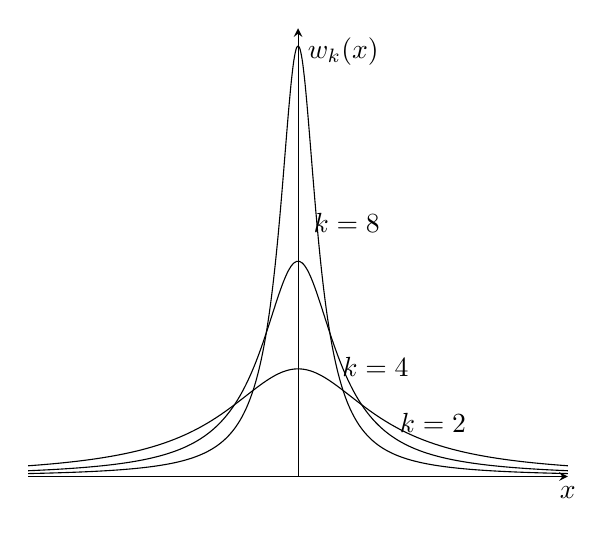
\begin{tikzpicture}
        \begin{axis}[
            axis lines = middle,
            xlabel = \(x\),
            ylabel = \(w_k(x)\),
            x label style = {anchor=north},
            xtick = {0},
            ytick= {0},
            ymin=0,
            ymax = 2.65,
            restrict y to domain=0:2.65
        ]
            \addplot[
                samples=200, 
                smooth,
                domain = -1.5:1.5
                ] 
                {2/(pi*(1+2^2*x^2))};
                \node at (axis cs:0.75, 0.32) {$k=2$};
            \addplot[
                samples=200, 
                smooth,
                domain = -1.5:1.5
                ] 
                {4/(pi*(1+4^2*x^2))};
                \node at (axis cs:0.43, 0.65) {$k=4$};
            \addplot[
                samples=200, 
                smooth,
                domain = -1.5:1.5
                ] 
                {8/(pi*(1+8^2*x^2))};
                \node at (axis cs:0.27, 1.5) {$k=8$};
        \end{axis}
    \end{tikzpicture}
    \caption{Mass Density;  eq. 3.3}
\end{figure}

If we let \(k \rightarrow \infty\), then the mass distribution approaches our idea of a point mass at \(x=0\). We would like to write
\begin{equation} \label{eq:deltaSeqLim}
    \delta(x) \overset{?}{=} \lim_{k\rightarrow \infty} w_k(x)
\end{equation}
where, \(\d(x)\) is the \df{Dirac delta function}. This "definition" feels intuitive, but it is not a rigorous definition of the Dirac delta function because the limit is infinite for \(x=0\). That is, the right-hand side is not a function. We instead define the Dirac delta function, \(\d(x)\), in the following way
\begin{equation}\label{eq:seqDef}
    \begin{split}
        \lim_{k\rightarrow \inf}\intR h(x)w_k(x)dx &= \intR h(x)\d(x)dx \\
        &= h(0)
    \end{split}
\end{equation}
and call any \(w_k(x)\) which has this property a \df{\(\d\)-sequence}. This way of defining the Dirac delta function is more rigorous while still being as intuitive as equation (\ref{eq:deltaSeqLim}). However, keep in mind that the delta function is not a function.

We would like to be able to check that a particular sequence \(w_k(x)\), is a \(\d-sequence\). We can do this by showing that equation (\ref{eq:seqDef}), holds for \(w_k(x)\). However, for certain, \(w_k(x)\), it is sufficient to show that \(\intR w_k(x)dx=1\).

\begin{definition}
    A function, \(f\), is \df[uniform continuity]{uniformly continuous} if for all \(\e>0\), a \(\d >0\) exists such that, if \(|a-b|<\d\), then \(|f(a)-f(b)|<\e\), for all \(a,b\in X\).
\end{definition}

\begin{theorem}\label{th:assertion}
    If \(w(x)\) is non-negative \(\intR w(x) dx = 1\), and \(w(x)=O(1/x^{1+\a})\) as \(|x| \rightarrow \inf\) with \(\a>0\), then \( w_k(x) \equiv kw(kx)\) is a \(\d\)-sequence.
\end{theorem}
\begin{proof}    
    We have
    \begin{equation}\label{eq:deltaseqProof1}
        \begin{split}
            \lim_{k\rightarrow \inf}\intR w_k(x)h(x) dx &= \underbrace{\lim_{k\rightarrow\inf} \intR w_k(x)[h(x)-h(0)]dx}_I+ \underbrace{\lim_{k\rightarrow\inf} \intR w_k(x)h(0)dx}_J.
        \end{split}
    \end{equation}
    Consider J,
    \begin{equation}
        \begin{split}
            J &= h(0) \lim_{k\rightarrow\inf} \intR kw(kx)dx\ \&\ \text{Let  }\xi =kx\\
            &=h(0){k\rightarrow \inf} \intR w(\xi) d\xi\\
            &= h(0).
        \end{split}
    \end{equation}
    Next, we wish to show that \(I=0\), so that the right hand side of equation (\ref{eq:deltaseqProof1}) is \(h(0)\). Let \(\epsilon > 0\), and since \(h\) is continuous at \(x=0\), there must exist a number \(\d>0\) such that \(|h(x)-h(0)|<\epsilon\) whenever \(|x-0|=|x|<\d\). Breaking up the integral \(I\),
    \begin{equation}
        \begin{split}
            I &= \underbrace{\lim_{k\rightarrow \inf} \int_{-\inf}^{-\d} w_k(x)(h(x)-h(0)) dx}_{I_1} + \underbrace{\lim_{k\rightarrow \inf} \int_{-\d}^{\d} w_k(x)(h(x)-h(0)) dx}_{I_2} \\ & + \underbrace{\lim_{k\rightarrow \inf} \int_{\d}^{\inf} w_k(x)(h(x)-h(0)) dx}_{I_3}.\\
        \end{split}
    \end{equation}
    Clearly, \( \lim_{k\rightarrow \inf} w_k(x)=0\), for each fixed \(x \neq 0\) , because \(w_k(x)=kw(kx)=O(k\cdot k^{-1-\alpha} |x|^{-1-\a}) = O(k^{-\a}) \rightarrow 0\) as \(k \rightarrow \inf\). 
    Since \(w_k(x)\rightarrow 0\) uniformly, over \(-\inf< x < -\d\) and \(\d < x < \inf \), then \(I_1=I_3 =0\). By the definition of uniform continuity \(|h(x)-h(0)|<\e\) whenever \(|x-0|=|x|<\d\). Because \(\e\) can be selected as small as we like, \(|h(x)-h(0)|=0\). As a result,
    \begin{equation*}
        \begin{split}
            I_2 &= \lim_{k\rightarrow \inf} \int_{-\d}^{\d} w_k(x)(0) dx\\
            &=0
        \end{split}
    \end{equation*}
    Thus, \(I=0\) and so 
    \begin{equation}
        \lim_{k\rightarrow \inf}\intR w_k(x)h(x) dx = h(0).
    \end{equation}

    
\end{proof}

\subsection{The Dirac Delta Function as a Generalized Function}
The Dirac delta function can also be defined as a generalized function. To understand this way of defining \(\d\), we will begin by defining some terms.

\begin{definition}
     A \df{closed region} is one that includes its endpoints.
\end{definition}

\begin{definition}
    The \df{support} of a function, \(f\), is the subset, \(\mathcal{S}\), of the domain of \(f\) such that for all \(x\in \mathcal{S}\), \(f(x) \neq 0\).
\end{definition}

\begin{definition}
    A function has \df{compact support} if the subset of its domain for which its range is non-zero is closed and bounded.
\end{definition}
We will call the space of infinitely differentiable functions with compact support \(\mathcal{D}\).

\begin{definition}
    \df[generalized function]{Generalized functions} are linear functionals that are uniformly continuous on \(\mathcal{D}\), such that all generalized functions have derivatives which are also generalized functions.
\end{definition}

We consider the following functional,
\begin{equation}\label{eq:generalizedFunction}
    \mathcal{F}(h) = \int_{-\infty}^{\infty} g(x)h(x)dx.
\end{equation}
This functional assigns a numerical value, \(\mathcal{F}(h)\), for each function \(h\) within the domain, \(\mathcal{D}\), of \(\mathcal{F}\).

\begin{example}
    Suppose \(\mathcal{F}(h)\) is the integral of \(h\) from \(\xi\) to \(\infty\).
    \begin{equation}
        \int_{\infty}^{\infty} g(x)h(x)dx = \int_{\xi}^{\infty} h(x) dx
    \end{equation}
    Then, \(g(x)\) is equivalent to the \df{Heaviside step function},
    \begin{equation}
        H(x) = \begin{cases}
            1, & x>0\\
            0, & x<0\\
            \frac{1}{2}, & x=0
        \end{cases}
    \end{equation}
    which is a function in the classical sense. \footnote{We have defined \(H(0)\) to be \(\frac{1}{2}\), which is a common convention. However, for our purposes, the value at any particular point is not important since we are only ever interested in integrating the function.}    
\end{example}

If \(\mathcal{F}(h)\) is \(h(0)\) so that
\begin{equation}\label{eq:introtodelta}
    \int_{-\infty}^{\infty}g(x)h(x) dx=h(0)
\end{equation}
then it can be shown that there is no function, \(g(x)\), which exists such that equation (\ref{eq:introtodelta}) is true for all functions, \(h(x)\), in the domain, \(\mathcal{D}\). We call \(g\) defined by equation (\ref{eq:introtodelta}) a generalized function, and in particular, it is the Dirac delta function. As such, \(\delta\) is defined in the following way.
\begin{equation}\label{eq:deltadef}
    \int_{-\infty}^{\infty} \delta(x)h(x) dx = h(0)
\end{equation}
for all \(h\in \mathcal{D}\).

Although \(\delta(x)\) has support at \(x=0\), it can be adjusted to have support at any point by shifting the argument. Thus, \(\delta(x-\xi)\) acts at \(x=\xi\),
\begin{equation}
    \int_{-\inf}^{\infty} \delta(x-\xi)h(x)dx = h(\xi).
\end{equation}

\begin{definition}
    We define the derivative of a generlaized function, \(g'\), in relation to \(g\) by performing integration by parts on
    \begin{equation}
            \intR g'(x)h(x) dx= g(x)h(x)\biggr\rvert_{-\infty}^{\infty} - \intR g(x)h'(x)dx.
    \end{equation}
\end{definition}
The integral term is fairly simple to interpret since it is of the same form as equation (\ref{eq:generalizedFunction}), but the boundary term is not as nice because it involves knowing the values of \(g\), which are never known. However, our restriction that \(h\) has compact support gives the intuition that it must vanish at infinity, and since we are integrating from \(-\inf\) to \(\inf\), the boundary term must be zero,
\begin{equation}
    \intR g'(x)h(x)dx = -\intR g(x)h'(x)dx.
\end{equation}
For the Dirac delta function, this means
\begin{equation}
    \begin{split} \label{eq:deltafirst}
        \intR \delta'(x-\xi)h(x)dx &= -\intR\delta(x-\xi)h'(x)dx\\
        &=-h'(\xi).
    \end{split}
\end{equation}


\begin{theorem} \label{th:deltad}
    The \(j\)th derivative of the Dirac delta function is defined by
    \begin{equation}
         \intR \delta^{(j)}(\xi-x)h(\xi)d\xi = (-1)^jh^{(j)}(x).
    \end{equation}
\end{theorem}
\begin{proof} We prove the statement by induction.\\
    \textbf{Base case:} Proven to be true for \(k\) = 1 in equation (\ref{eq:deltafirst}).\\
    \textbf{Induction step:} Let \(k \in \mathbb{N}\) and suppose the statements holds for some \(k\geq 1\). Then,
    \begin{align*}
        \intR \delta^{(k+1)}(\xi-x)h(\xi)d\xi &= \d^{(k)}(\xi-x)h(\xi)\bounds{-\inf}{\inf}-\intR \delta^{(k)}(\xi-x)h'(\xi)d\xi\\
        &=-\intR \delta^{(k)}(\xi-x)h'(\xi)d\xi\\
        &=-(-1)^{k}(h')^{(k)}(x)\\
        &=(-1)^{k+1}h^{(k+1)}(x)
    \end{align*}
\end{proof}

Note that because of the discontinuity in \(H(x-\xi)\) at the point \(x=\xi\), the derivative of \(H\) does not exist as an ordinary function. However, the previous method does allow us to find \(H'(x-\xi)\) as a generalized function, 
\begin{equation}
    \begin{split}
        \intR H'(x-\xi)h(x)dx &= -\intR H(x-\xi)h'(x)dx\\
        &=-\int_{\xi}^{\infty}h'(x)dx \\
        &= h(\xi).
    \end{split}
\end{equation}
Since
\begin{equation}
    \intR \delta(x-\xi)h(x)dx=h(\xi)
\end{equation}
it must be the case that, in the sense of generalized functions,
\begin{equation}
    H'(x-\xi) = \delta(x-\xi).
\end{equation}
Such equalities between generalized functions, as seen in (3.18), are understood in the sense that if some \(h\) in \(\mathcal{D}\) is multiplied through, and we integrate over \((-\infty, \infty)\) then the result will hold. To wit, we consider generalized functions, \(g_1\) and \(g_2\), to be equal if, for all \(h\in \mathcal{D}\),
\begin{equation}
    \intR g_1(x)h(x)dx = \intR g_2(x)h(x)dx.
\end{equation}

Notice that for all \(n > 0\)
\begin{equation}
    x^n\delta(x)=0
\end{equation}
as a result of
\begin{equation}
    \intR x^n\delta(x)h(x)dx=[x^nh(x)]|_{x=0} = 0.
\end{equation}

\begin{example}
    We would like to show that the sequence
    \begin{equation*}
        w_k(x) = \begin{cases}
            k, &  0<x<\frac{1}{k}\\
            0, &x\leq 0 \text{ or } x \geq \frac{1}{k}
        \end{cases}
    \end{equation*}
    is a \(\d\)-sequence using theorem (\ref{th:assertion}). It is clear that \(w_k(x)\geq 0\)  for all \(x\) and \(w(x)=O(1/|x|^{1+\a})\) as \(|x| \rightarrow \inf\) with \(\a>0\) since it is zero when \(x \leq 0\) or \(x \geq 1/k\). Lastly, we must show that the area under \(w(x)\) is 1. Choosing \(w(x)\) so that \(kw(kx)=w_k(x)\)
    \begin{equation*}
        w(x)=\begin{cases}
            1,& 0<x<1\\
            0,& x\leq0 \text{ or } x \geq 1.
        \end{cases}
    \end{equation*}
    Integrating:
    \begin{equation}
        \begin{split}
            \intR w(x) dx &= \int_{-\inf}^{0} 0 dx +\int_0^1 1 dx + \int_{1}^{\inf} 0 dx\\
            &=\int_0^1 1 dx\\
            &=1
        \end{split}
    \end{equation}
\end{example}

\begin{example}
    We would like to show that the sequence,
    \begin{equation}
        w_k(x) = \begin{cases}
            -k, &|x|<\frac{1}{2k}\\
            2k, &\frac{1}{2k} \leq |x| \leq \frac{1}{k}\\
            0, &|x|> \frac{1}{k},
        \end{cases}
    \end{equation}
    is a delta sequence. Theorem (\ref{th:assertion}) does not apply in this case because \(w_k(x)\) is negative for some values of \(x\) so we should instead show 
    \begin{equation}
        \lim_{k\to \inf}\intR w_k(x) h(x) dx = h(0).
    \end{equation}
    To begin, we break up the integral 
    \begin{equation}
        \begin{split}
            \lim_{k\to \inf}\intR w_k(x) h(x) dx &= \lim_{k\to \inf}\int_{-\frac{1}{k}}^{-\frac{1}{2k}} 2kh(x)dx - \lim_{k\to \inf}\int_{-\frac{1}{2k}}^{\frac{1}{2k}} kh(x)dx \\
            &+ \lim_{k\to \inf}\int_{\frac{1}{2k}}^{\frac{1}{k}} 2kh(x)dx
        \end{split}
    \end{equation}
    
    Consider each integral. Let \(-\frac{1}{k}<\xi<-\frac{1}{2k}\). By the mean value theorem
    \begin{equation*}
        \begin{split}
            \lim_{k\to \inf}\int_{-\frac{1}{k}}^{-\frac{1}{2k}} 2kh(x)dx &= \lim_{k\to \inf}  \left( \left(-\frac{1}{2k} + \frac{1}{k}\right) 
            \cdot 2k\cdot h(\xi)\right) \\
            &=h(0).
        \end{split}
    \end{equation*}

    \begin{equation*}
        \begin{split}
            \lim_{k\to \inf}\int_{-\frac{1}{2k}}^{\frac{1}{2k}} -kh(x)dx &= \lim_{k\to \inf}  \left( \left(\frac{1}{2k} + \frac{1}{2k}\right) 
            \cdot -k\cdot h(\xi)\right) \\
            &=-h(0).
        \end{split}
    \end{equation*}

    \begin{equation*}
        \begin{split}
            \lim_{k\to \inf}\int_{\frac{1}{2k}}^{\frac{1}{k}} 2kh(x)dx &= \lim_{k\to \inf}  \left( \left(\frac{1}{k} - \frac{1}{2k}\right) \cdot 2k\cdot h(\xi)\right) \\
            &=h(0).
        \end{split}
    \end{equation*}
    The last step for each integral follows from the fact that as \(k \to \inf\) \(\xi\to 0\). Adding each integral shows that
    \begin{equation*}
        \lim_{k\to \inf}\intR w_k(x) h(x) dx = h(0).
    \end{equation*}
\end{example}

\begin{example}
    We would like to show that \(e^x\d(x)=\d(x)\). To begin with, we integrate \(e^x\d(x)f(x)\) and would like to show that this is equal to \(f(0)\) to satisfy the generalized function definition of the delta function.
    \begin{equation}
        \begin{split}
            \intR e^x\d(x)f(x)dx &= \intR \d(x)\underbrace{e^xf(x)}_{g(x)}dx\\
            &=\intR \d(x)g(x)dx\\
            &=g(0)\\
            &=e^0f(0)\\
            &=f(0)\\
        \end{split}
    \end{equation}
    Therefore
    \begin{equation}
        \intR e^x\d(x)f(x)dx = \intR \d(x)f(x)dx
    \end{equation}
\end{example}
\begin{example}
    We would like to show that \(\frac{d^4}{dx^4}|x|^4 = 12\d(x)\). Note that \(|x|=2xH(x)-x\). We begin by manipulating \(|x|^3\) into a more convenient form.
    \begin{equation}
        \begin{split}
            |x|^3 &= (2xH(x)-x)^3\\
            &=x^3(2H(x)-1)^3\\
        \end{split}
    \end{equation}
    Next, it is useful to simplify.\\
    Note: \(H^n(x)=H(x)\), \(n\in\mathbb{N}\).
    \begin{equation}
        \begin{split}
            (2H(x)-1)^3 &= (2H(x))^3-3(2H(x))^2+3(2H(x))-1\\
            &=8H(x)-12H(x)+6H(x)-1\\
            &=2H(x)-1
        \end{split}
    \end{equation}
    Finally, we the fourth derivative.
    \begin{equation}
        \begin{split}
            D^4(x^3(2H(x)-1)) &= D^3(3x^2(2H(x)-1) +2x^3\d(x))\\
            &=D^3(3x^2(2H(x)-1))\\
            &= D^2(6x(2H(x)-1) + 6x^2\d(x))\\
            &=D^2(6x(2H(x)-1))\\
            &= D(12(H(x)-1) + 12x\d(x))\\
            &= D(12(H(x)-1))\\
            &= 12\d(x)
        \end{split}
    \end{equation}
\end{example}

\section{The Method of Green's Functions}
\setcounter{example}{0}
A Green's function is the solution to a differential equation of the form
\begin{equation} \label{eq:greensdef}
    \opp{L^*} G = \delta.
\end{equation}
By making use of some of the delta function's unusual properties, Green's functions can be used to solve nonhomogeneous linear differential equations.

To find the solution to the linear differential equation
\begin{equation} \label{eq:4.2}
    \opp{L}u=\phi,
\end{equation}
we start by finding the formal adjoint as in equation (\ref{eq:adjoint}). If instead of \(v\), we use \(G\) to represent the Green's function, and we replace \(x\) with a dummy variable \(\xi\), we are left with an equation of the form
\begin{equation} \label{eq:greenadjoint}
    \intl G(\xi, x)\opp{L}u(\xi) d\xi = \bterms + \intl u(\xi)\opp{L^*}G(\xi,x) d\xi.
\end{equation} 
It follows from equation (\ref{eq:g reensdef}) that the we can replace \(\opp{L^*}G\) with \(\d\), and from equation (\ref{eq:4.2}) that we can replace \(\opp{L}u\) with \(\phi\). 
\begin{equation}
    \begin{split}
        \intl G(\xi,x)\phi(\xi) d\xi &= \bterms + \intl u(\xi)\d(\xi-x) d\xi\\
        &=\bterms + u(x).
    \end{split}
\end{equation}
Therefore, if we choose boundary conditions for \(G\) such that the boundary terms do not depend on \(u\) and we are able to find \(G\), then finding \(u\) is reduced to a problem of integrating \(G\phi\). 

To illustrate the key ideas of the method, we will consider several examples which begin simply and become more complex. Each example will be concerned with a key concept in implementing the method of Green's functions.
\begin{example}
    \textit{Loaded String}
    
    Consider the boundary value problem
    \begin{equation}
        u''(x) = \phi(x);\quad u(0)=u(1)=0
    \end{equation}
    where \(\phi(x)\) is prescribed. \textbf{EXPLAIN LOADED STRING WITH DIAGRAM}. 
    
    We must first find the formal adjoint \(\opp{L^*}\) as in equation (\ref{eq:greenadjoint}). 
\end{example}


\appendix

\newpage
\section{Tabular Integration by Parts}
    One can use a table to perform repeated integration by parts quickly. Suppose we would like to use integration by parts to change the integral of \(v(x)u^{(4)}(x)\) into boundary terms plus the integral of \(v^{(4)}(x)u(x)\). In the first column, we write \(v(x)\) and its derivatives beneath it. In the second column, we write \(u^(4)(x)\) and its anti-derivatives beneath it. At the end of this process, the table should look as follows.
    \begin{table}[H]
        \centering
        \begin{tabular}{c|c}
            \(v(x)\) & \(u^{(4)}(x)\)\\
            \(v'(x)\) & \(u'''(x)\)\\
            \(v''(x)\) & \(u''(x)\)\\
            \(v'''(x)\) & \(u'(x)\)\\
            \(v^{(4)}(x)\) &\(u(x)\)
        \end{tabular}
    \end{table}
    Next, each row of the left column is given alternating signs, beginning with positive.
    \begin{table}[H]
        \centering
        \begin{tabular}{c|c}
            \(+v(x)\) & \(u^{(4)}(x)\)\\
            \(-v'(x)\) & \(u'''(x)\)\\
            \(+v''(x)\) & \(u''(x)\)\\
            \(-v'''(x)\) & \(u'(x)\)\\
            \(+v^{(4)}(x)\) &\(u(x)\)
        \end{tabular}
    \end{table}
    Next we multiply diagonal terms and add each product.
    \begin{figure}[H]
        \centering
        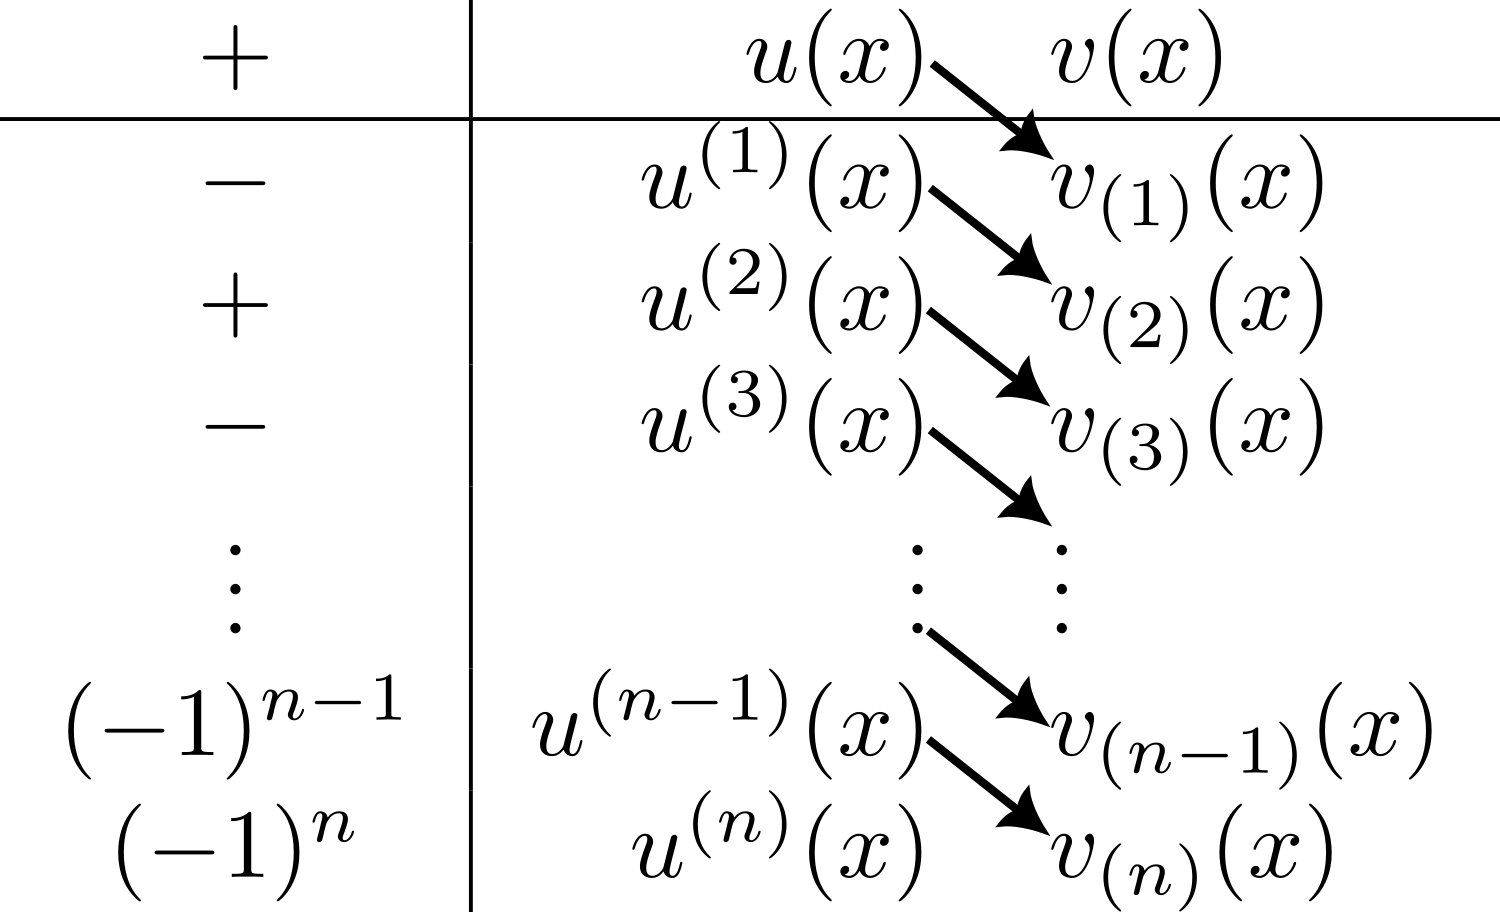
\includegraphics{include/tabular-boundary.png}
    \end{figure}
    These are the boundary terms. Lastly, we multiply the bottom terms together. 
    \begin{figure}[H]
        \centering
        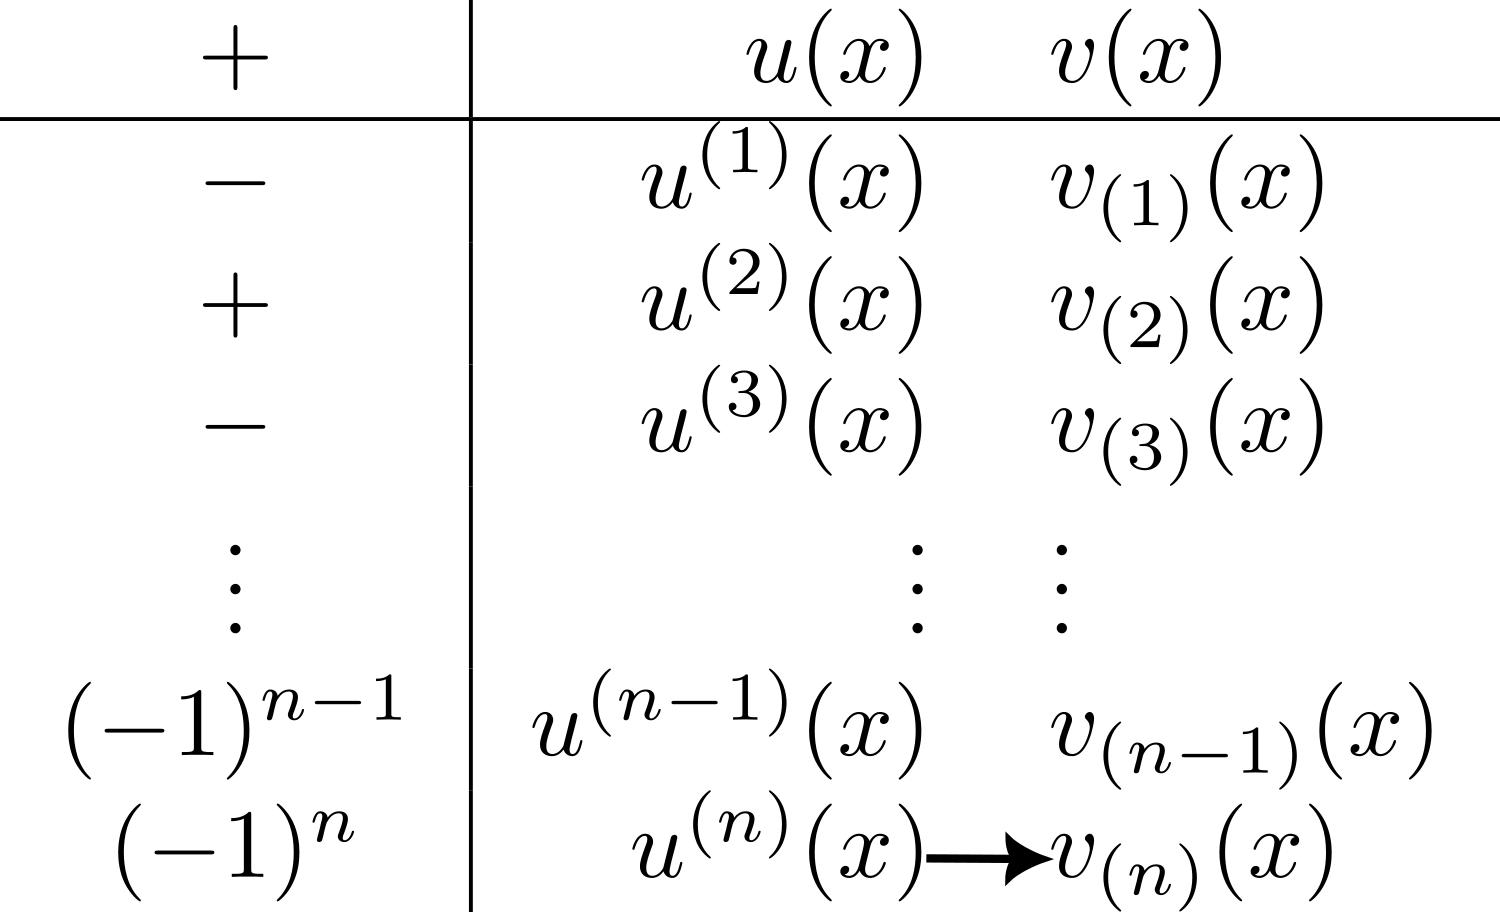
\includegraphics{include/tabular-integrand.png}
    \end{figure}
    This is the integrand. The result at the end of this is 
    \begin{equation}
        \intl v(x)u^{(4)}(x) dx = (v(x)u'''(x) - v'(x)u''(x) + v''(x)u'(x)-v'''(x)u(x))\biggr\rvert_\mathrm{a}^\mathrm{b} + \intl v^{(4)}(x)u(x) dx.
    \end{equation}
\section{The Mean Value Theorem}
    The mean value theorem states that for all \(f:[\lima,\limb]\to \mathbb{R}\) such that \(f\) is continuous on \([\lima,\limb]\), and differentiable on \((\lima, \limb)\), then 
    \begin{equation}
        \exists c \in (\lima, \limb) : f'(\text{c}) = \frac{f(\limb)-f(\lima)}{\limb-\lima}
    \end{equation}
    and thus,
    \begin{equation}
        f'(c)(\limb-\lima) = f(\limb)-f(\lima)
    \end{equation}
    By integrating \(f'(x)\) , we see that
    \begin{equation}
        \begin{split}
            \int_\lima^\limb f'(x) dx &= f(\limb)-f(\lima)\\
            &=f'(\text{c})(\limb-\lima)
        \end{split}
    \end{equation}
\section{Big O Notation}
Big O notation is used to describe the limiting behavior of a function as the argument tends to some value or infinity. By \(f(x)=O(g(x)\) as \(x\to x_0\) we mean that \(\frac{f(x)}{g(x)}\) is bounded as \(x\to x_0\). For example 
\begin{equation}
    \sin 6x = O(1) \text{ as } x\to \inf.
\end{equation}

\addcontentsline{toc}{section}{References}

\bibliographystyle{alpha}
\bibliography{include/biblio}
Greenberg, Michael D. Applications of Green’s Functions in Science and Engineering. Dover

Publications, 2015.\\
Roach, G. F. Green’s Functions. Cambridge University Press, 1982.


\printindex

\end{document}
